\chapter{Prologue}
\label{ch:prologue}

The quantity of data, information, and knowledge in the biomedical domain is increasing at an unprecedented rate — with no signs of deceleration.
Even with the assistance of information retrieval technologies, it is overwhelming, if not impossible, for individuals or groups of researchers to be knowledgeable of the state-of-the-art in any but an incredibly specific topic.
Besides their obvious increases in volume and velocity, data are also increasing in variety as multi-modal and multi-scale experiments grow more important in the investigation of complex diseases.

As experiments' complexities grow, so does the intellectual and temporal burden of analysis and interpretation.
Developing systematic and reproducible methods to reduce this burden first requires the formalization and assembly of knowledge in a computable form.
The publications in this thesis build towards leveraging and improving previously existing methodologies for extracting, formalizing, and storing biological knowledge to support the development and application of algorithms towards unraveling the complex biology of disease and proposing new therapies.

Before presenting the publications included in this thesis, background is given on several topics present through each including the nomenclature of entities in the biomedical literature, the techniques and formalisms used for biomedical knowledge graphs, algorithms appropriate for analyzing biomedical knowledge graphs, and finally, their applications.

\section{Nomenclature}

The first two sections of the introduction examine the organization of biomedical knowledge, and several of the challenges faced during the process.
These challenges span from unifying the nomenclature of biologically relevant entities used in the published biomedical literature to extracting the biological knowledge and context surrounding those entities.

\subsection{Issues with Gene Nomenclature}

The nomenclature of genes and gene products is a particularly egregious example of poor nomenclature within the biomedical domain.
Genes often have several names as well as several incomprehensible acronyms, or gene symbols.
For example, the \ac{HGNC}~\cite{Yates2017} and Entrez Gene~\cite{Maglott2011} database list that the human gene microtubule associated protein tau (hgnc:HGNC:6893, ncbigene:4137) has previously been named the G protein
$\beta1$/$\gamma2$ subunit-interacting factor 1 and the protein phosphatase 1,
regulatory subunit 103.
Like with many genes, it is often acronymized to MAPT in text, but it has additionally been previously referenced with DDPAC, FLJ31424, FTDP-17, MAPTL, MGC13854, MTBT1, MTBT2, MSTD, PPND, and PPP1R103.

Neither genes' names nor their gene symbols convey their host species, which leads to further ambiguities in articles discussing orthologs in model organisms.
The organization responsible for mouse gene nomenclature, \ac{MGI}~\cite{Blake2017}, names the mouse orthologous gene as microtubule-associated protein tau (mgi:MGI:97180, ncbigene:17762) and lists the gene symbol as Mapt.
In this example, the name varies from the human ortholog with the introduction of a hyphen between "microtubule" and "associated."
The gene symbol differs only in capitalization.
Similarly, the organization for rat genome nomenclature, the \ac{RGD}~\cite{Shimoyama2015}, names the rat orthologous gene as microtubule-associated protein tau (rgd:69329; ncbigene:29477)---exactly as in \ac{MGI}.
While these orthologs from common model organisms have had related names, organisms with genetic drift such as Zebrafish have several orthologs named microtubule-associated protein tau a (zfin:ZDB-GENE-081027-1) and microtubule-associated protein tau b (zfin:ZDB-GENE-081027-2) whose gene symbols are listed as mapta and maptb, respectively.
Other orthologs to human microtubule-associated protein tau can be found in Homologene (homologene:74962), Ensembl~\cite{Zerbino2018}, \ac{HGNC}, \ac{MGI}, PomBase, \ac{RGD}, Xenbase, and \ac{ZFIN}.
The \ac{HCOP}~\cite{Wright2005} aggregates these and several other sources of curated and predicted orthologies.

\subsection{Nomenclature Consortia of Genes and Proteins}

Most biologically relevant named entities have many names.
For example, many genes were independently discovered and characterized in different labs and therefore named differently.
As resources for exchanging genomic and protein sequences have become more ubiquitous in the last three decades since the inception of the Entrez gene database in 1991 and the \ac{HGNC} in 1996, it has become easier to reduce those duplicates.
However, this does not solve the problem of establishing a canonical name for each entity.
As stated in the previous section, several committees and consortia have formed to standardize the nomenclature used for genes for each species (Table~\ref{tab:gene_nomenclature_databases}).

\begin{table}
    \centering
    \caption{Example model organism gene nomenclature databases}
    \label{tab:gene_nomenclature_databases}
    \begin{tabular}{ l l l }
        Organism & Database & Reference \\
        \hline
        Human & \ac{HGNC} &\cite{Yates2017} \\
        Vertebrae & VGNC &\cite{Yates2017} \\
        Mouse & MGI &\cite{Blake2017} \\
        Rat & RGD &\cite{Shimoyama2015} \\
        Zebrafish & ZFIN &\cite{Howe2013}  \\
        Drosophila (fly) & FlyBase &\cite{Thurmond2019}\\
        Xenopus (frog) & Xenbase &\cite{Karimi2018}  \\
        Yeast & SGD &\cite{Cherry2012} \\
        - & Entrez Gene &\cite{Maglott2011}  \\
    \end{tabular}
\end{table}

\subsection{Nomenclature Consortia of Other Entities}

Besides gene nomenclature, there are several other biologically relevant physical entities and higher-order processes that have have the same issues in nomenclature.
Further, for higher-order processes like pathways, mechanisms, and biological processes, it not only remains unclear what to name each example, but where their boundaries lie.
However, deference to entities beyond genes and proteins is required to fully describe complex biology.
Thus, several groups have attempted to standardize and control the nomenclature of these entities (Table~\ref{tab:other_nomenclature_databases}).

\begin{table}
    \centering
    \caption{Example entity types of interest in the biomedical domain and corresponding nomenclature sources}
    \label{tab:other_nomenclature_databases}
    \begin{tabular}{ l l }
        Entity Type & Resources \\
        \hline
        Transcripts & Ensembl, miRBase \\
        Proteins & UniProt \\
        Protein Families & InterPro, neXtProt, FamPlex, ExPASy, Signor \\
        Protein Complexes & Complex Portal, FamPlex, Signor, Gene Ontology \\
        Biological Processes & Gene Ontology MeSH \\
        Pathways & Reactome, WikiPathways, KEGG \\
        Conditions and Phenotypes & Disease Ontology, Human Phenotype Ontology, MeSH
    \end{tabular}
\end{table}

\subsection{Practical Considerations in Named Entity Recognition}

Besides further synonyms and morphological variations, Bachman \textit{et al.}~\cite{Bachman2018} outlined several affixes corresponding to post-translational modification state, experimental context, or other categories (Table~\ref{tab:affix_categories}).

\begin{table}
    \centering
    \caption{Examples of affix categories in the FamPlex ontology adapted from Table 2 of~\cite{Bachman2018}}
    \label{tab:affix_categories}
    \begin{tabular}{ l l }
        Affix Category & Example \\
        \hline
        Experimental context & eGFP-\{Gene name\} \\
        Protein state & phospho-\{Gene name\} \\
        Inhibitor & shRNA-\{Gene name\} \\
        Generic descriptor & Proto-oncogene \{Gene name\} \\
        Species & mmu-\{Gene name\} \\
        mRNA grounding & \{Gene name\} mRNA
    \end{tabular}
\end{table}

Bachman \textit{et al.} also considered issues with recognizing proteins, protein families, and protein complexes~\cite{Bachman2018}.
The biomedical literature often references multi-protein families (e.g., RAS, AKT) and multi-subunit complexes (e.g., NF-kB, AP-1) rather than their constituent proteins.
For example, the protein family of phospholipase C enzymes, more commonly referenced as PLC, contains not only individual genes (e.g., PLCE1), but also subfamilies such as PLCG, which contains the genes PLCG1 and PLCG2.
The NF-kB complex comprises five proteins (i.e., RELA, RELB, REL, NFKB1, and NFKB2) and poses the further challenge of how named entities should be interpreted after recognition.

\subsection{Automating Named Entity Recognition}

In practice, automating the process of recognizing named entities has three major tasks: coreference resolution, \ac{NER}, and entity linking.

\subsubsection*{Coreference Resolution}

During the process of coreference resolution, antecedents or anaphors are identified and connected to their preceding or succeeding words or phrases.
In the example "The EGFR belongs to a family of protein-tyrosine kinase receptors. It is activated by the binding of EFG.", coreference resolution identifies that the subject of the second sentence, \textit{it}, refers to EGFR.
There are several classical rule-based coreference resolution algorithms including the syntax-based Hobbs theory~\cite{Hobbs1978}, discourse-based centering theory~\cite{Brennan1987}, and syntactic knowledge-based RAP algorithm~\cite{Brennan1987}.
However, recent improvements to coreference resolution have focused on four categories of machine learning techniques: mention-pair models~\cite{Soon2001,Ng2002,Bengtson2008}, entity-mention models~\cite{Luo2004,Yang2004,Yang2008}, mention-ranking models~\cite{Lee2011,Denis2007,Rahman2009,martschat2015}, and cluster-ranking models~\cite{Rahman2011,Ma2014,Clark2016}.
Recent work has focused on using recurrent neural networks with architectures such as the bi-directional long-short-term memory~\cite{Li2018} and variants such as the bi-directional long-short-term memory conditional random field~\cite{Giorgi526244}.

\subsubsection*{Named Entity Recognition}

During the process of \ac{NER}, words or phrases are identified to have domain-specific, non-trivial meaning.
In the biomedical domain, \ac{NER} is used to identify proteins~\cite{Hsu2008,Leaman2008, Hakenberg2011,Wei2015}, chemicals~\cite{Leaman2015,Corbett2018,Giorgi526244}, diseases~\cite{Leaman2013,Giorgi526244}, taxa~\cite{Gerner2010,Wei2012}, and other entity types listed in Table~\ref{tab:other_nomenclature_databases}.

Unlike the difference between machine learning models of coreference resolution with rule-based or natural language processing models, \ac{NER} workflows often contain a mixture of preprocessing steps, rule-based feature generation, statistical models, machine learning models, and postprocessing steps.
For example, Lee \textit{et al.}~\cite{Lee2015} defined six feature classes for training a disease recognition model using a conditional random field:
\begin{enumerate}[noitemsep]
    \item Morphological features that contained the original tokens, the corresponding stemmed tokens, and their affixes
    \item Features based on their terminology of trigger words related to diseases, body parts, and human ability
    \item Classical part-of-speech features.
    \item Transformation of the original tokens to remove continued vowels, such as the superfluous ``u'' in the british spelling of tumour.
    \item Features using a dictionary lookup on the \ac{MEDIC}~\cite{Davis2012}.
    \item Annotated abbreviations using BIOADI~\cite{Kuo2009}.
\end{enumerate}

Other workflows have opted to use end-to-end machine learning following the advent of word embedding techniques such as word2vec~\cite{Mikolov2013} and GloVe~\cite{Pennington2014} and deep learning techniques like the long-short-term memory conditional random field architecture~\cite{Lample2016}.
Both variants require carefully constructed and annotated corpora such as GENIA~\cite{Kim2003} or those provided by the various BioCreative challenges (\url{https://biocreative.bioinformatics.udel.edu}).
With machine learning techniques, the annotations become more important as they are also necessary for supervised learning.

\subsubsection*{Entity Linking}

During the process of entity linking (i.e., normalization, grounding), named entities that have been recognized in the previous step (\ac{NER}) are \textit{grounded} to terms in controlled vocabularies or databases.
For example, this means that the token MEK1 should be recognized as a synonym of the MAP2K1 gene and subsequently grounded with the \ac{HGNC} identifier hgnc:HGNC:6840, Entrez Gene identifier ncbigene:5604, UniProt identifier uniprot:Q02750, and any other desired equivalent identifiers.
Practically, mappings between equivalent terms in databases are manually curated by database maintainers and data stewards.
As more of the nomenclatures, terminologies, and taxonomies useful to the bioinformatics community move towards ontological formats like the \ac{OWL} and the \ac{OBO} standard, these mappings become more reusable.
Concurrently, tools like the \ac{EBI} \ac{OLS}~\cite{Cote2006} and emerging \ac{EBI} Ontology Xref Service (\url{https://www.ebi.ac.uk/spot/oxo}) have been able to provide the community with technical solutions for storing, indexing, and looking up information about these terms.

\subsection{Beyond Nomenclature and Standards for Reference}

The ambiguity of nomenclature in the biomedical domain presents several problems, especially as the acceleration of publication makes automated information extraction more relevant.

Anecdotally, there are few real-world data sets using \ac{HGNC} gene symbols as identifiers that can be directly and fully mapped to \ac{HGNC} entries.
This is because the gene symbols listed by \ac{HGNC} are notoriously unstable---hundreds or thousands change per year (Figure~\ref{fig:gene_symbol_half_life}).
These changes might be due to the splitting of a single gene entry into a family of entries, the merging of disparate genes that were the same, or deprecation of previous nomenclature.
Further, Figure~\ref{fig:gene_symbol_half_life} provides an underestimate of the impact of this issue due to the fact that the \ac{HGNC} only lists the most recent date of change for each gene symbol.

\begin{figure}
    \captionsetup{format=plain}
    \makebox[\textwidth]{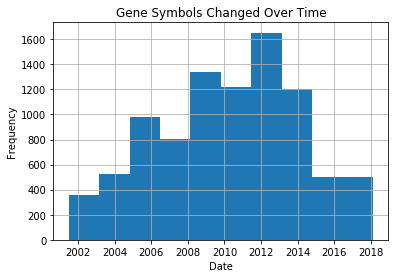
\includegraphics[width=100mm]{figures/gene_symbol_half_life.png}}
    \caption[HGNC Gene Symbol Half Lives]{The frequency by which \ac{HGNC} gene symbols change over time. This figure was generated with the Jupyter notebook available at~\cite{Hoyt2018GeneHalfLife}.}
    \label{fig:gene_symbol_half_life}
\end{figure}

The \ac{MIRIAM}~\cite{Laibe2007} standard was proposed in order to standardize the way named biological entities are referenced in models and databases in order to address the issues with reproducibility arising from the previously described phenomena in natural language as part of the Minimum Information for Biological and Biomedical Investigations~\cite{Taylor2008}.
At its core, \ac{MIRIAM} posits that instead of imprecise names, the bioinformatics community should shift towards using identifiers with five properties: unique (i.e.,\ never assigned to two different entities), perennial (i.e.,\ never changes and is permanent), standards compliant (i.e.\ conform to standards like \ac{URI}, \ac{CURIE}, etc.), free to use, and resolvable (i.e.,\ can be transformed into locations of appropriate online resources).
Note that in the previous section, identifiers were written using the \ac{CURIE} style (e.g., an identifier prefixed with a namespace).
Curiously, the \ac{HGNC} identifier includes a redundant mention of the namespace within the identifier.
Further standardization of redundant \ac{CURIE}s is discussed in Chapter~\ref{ch:bio2bel}.

As Figure~\ref{fig:gene_symbol_half_life} suggests, \ac{HGNC} gene symbols are not perennial and are not \ac{MIRIAM} compliant.
However, even a decade after the proposal of \ac{MIRIAM}, many databases have not yet shifted away from storing and annotating data with \ac{HGNC} gene symbols to using more stable \ac{HGNC} identifiers.

Unfortunately, there has been few or no concerted efforts from authors and publishers to better annotate articles with identifiers for named entities.
Thus, \ac{NER} and entity linking remain relevant as ever, especially due to the increasing volume of literature describing increasingly complex biology across many scales.

\section{Formalization of Knowledge}

\subsection{Abstraction of Methodological, Conceptual, and Factual Knowledge}

The most abstract level of knowledge, methodological knowledge, describes the formalisms through which knowledge can be represented.
The two most common schemata for methodological knowledge are \ac{RDFS} and \ac{OWL}.
They provide the faculty to describe the middle level, conceptual knowledge, which encodes the classes, relations, and constraints relevant to a given domain.
The most common conceptual knowledge formats in the biomedical domain are \ac{BioPAX}, \ac{SBML}, and \ac{BEL}.
The most concrete level is factual knowledge, which consists of instances of these classes and relationships~\cite{Marchetti2008}.
These abstractions are illustrated in Figure~\ref{fig:knowledge_types}.

\begin{figure}
    \captionsetup{format=plain}
    \makebox[\textwidth]{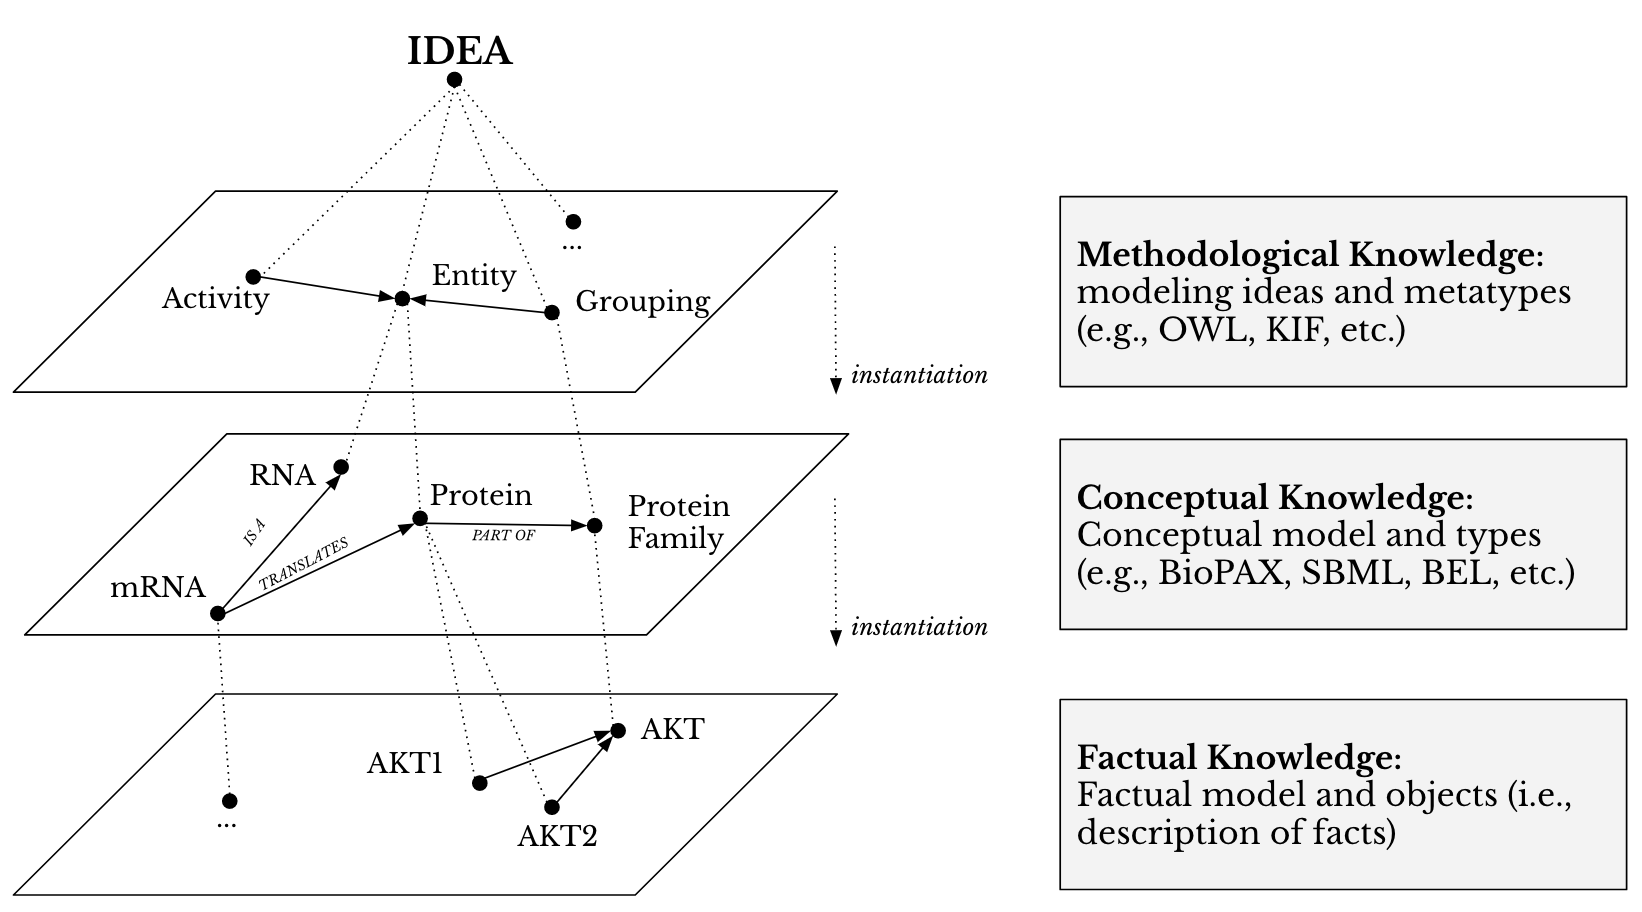
\includegraphics[width=160mm]{figures/knowledge_types.png}}
    \caption[Levels of Knowledge Abstraction]{The interplay of the three levels of knowledge abstraction in an example from the biological domain.}
    \label{fig:knowledge_types}
\end{figure}

\subsection{Realizations}

\subsubsection{Resource Description Framework Schema}

\ac{RDF} uses triples of subjects, predicates, and objects to represent relations between concepts.
Each resource in a triplet is backed by an \ac{IRI}.
While its simple format grants it huge expressive power, \ac{RDF} lacks structure or domain specificity.
\ac{RDFS} is a set of concepts and predicates appropriate for describing knowledge at the conceptual level.
Included are predicates for asserting class hierarchies (rdfs:subClassOf), asserting memberships (rdf:type), describing the domain and range of predicates (rdfs:domain, rdfs:range), and representing epistemological concepts such as classes, literals, and other data types~\cite{Beckett2014}.
RDF and RDFS are supported by most popular programming languages with packages to serialize and deserialize RDF in a variety of formats (e.g., \ac{XML}, N-Triples, turtle, etc.) and reason over \ac{RDFS}.

\subsubsection{Web Ontology Language}

Like \ac{RDFS}, \ac{OWL} consists of the methodological knowledge for modeling domain-specific knowledge.
Its most simple form, \ac{OWL} Lite, enables the representation of classes, their properties, relations, and constraints.
The most common form, \ac{OWL} \ac{DL}, contains the additional expressive power of descriptive logic over which inferences can be made.
The most expressive form, \ac{OWL} Full, removes the remaining restrictions on \ac{OWL} \ac{DL} but paradoxically becomes undecidable and hinders automatic reasoning~\cite{Marchetti2008}.

\begin{figure}
    \captionsetup{format=plain}
    \makebox[\textwidth]{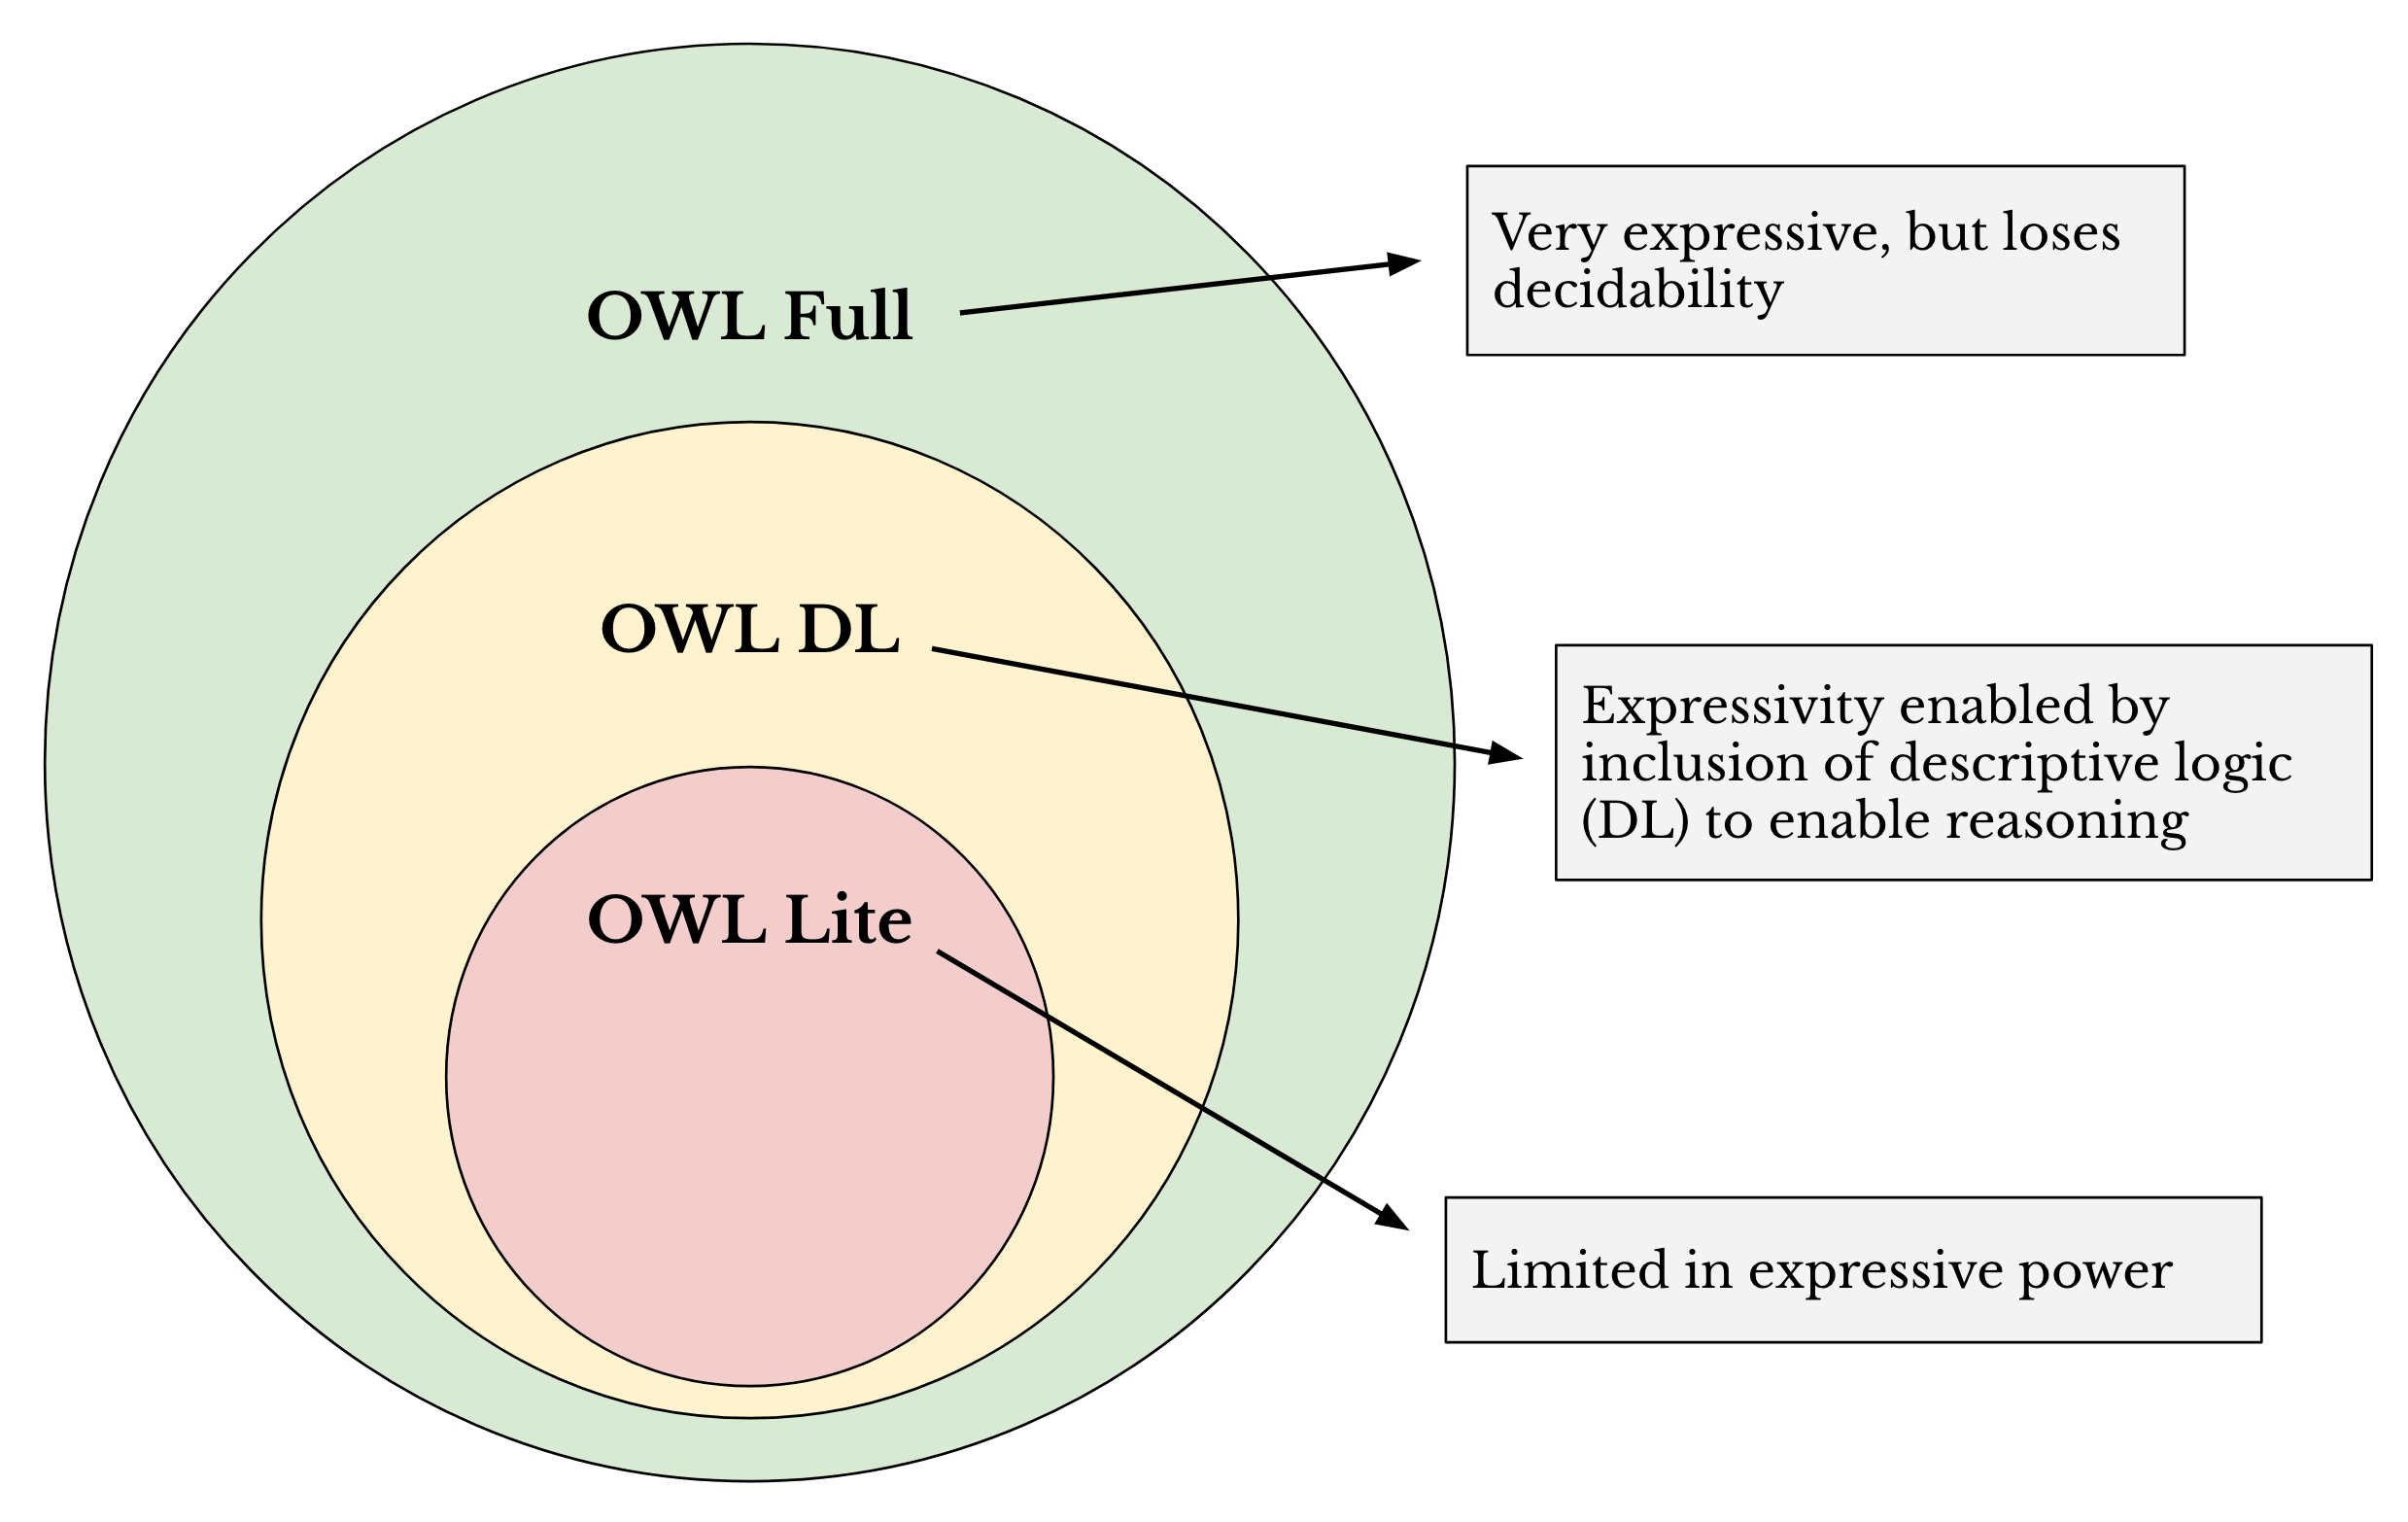
\includegraphics[width=160mm]{figures/owl_types.png}}
    \caption[Descriptive Levels of OWL]{The expressive levels of OWL ontologies. Adapted from~\cite{Marchetti2008}.}
    \label{Fig:owl_types}
\end{figure}

\subsubsection{OBO}

As the usage of ontologies began to percolate into the biomedical domain, Ashburner and Lewis proposed the \ac{OBO} standard~\cite{Ashburner2003} to encourage the standardization of formats and identifiers, to promote openness and community feedback, and to organize information in logical units.
The OBO Foundry~\cite{Smith2007} has emerged as a central repository that has successfully supported collaboration such as the collation of several previously disparate ontologies into the Cell Line Ontology~\cite{Sarntivijai2014}.
Because the syntax of \ac{OBO} is not directly compatible with \ac{OWL}, several converters have been exist to further support the integration of \ac{OBO} with other aspects of the Semantic Web.

\subsection{Standardized Curation of Biological Pathways}

As biological knowledge is generated from experiments or extracted from the literature it must be stored in a standard format to be generally useful.
This section describes several of those formats and their applicability domains.

\subsubsection{Biological Pathways Exchange Language}

\ac{BioPAX} uses \ac{OWL} to define the conceptual knowledge in the domain of biological pathways on the molecular and cellular level.
Its ability to collect and index metabolic, signaling, molecular, gene-regulatory, and genetic interaction networks makes it an ideal exchange format for the growing number of pathway databases with varying specificities in regards to target organisms and disease indications~\cite{Demir2010}.

This was realized with the aggregation of several pathway and interaction databases (e.g., BindingDB~\cite{Gilson2016}, DrugBank~\cite{Law2014}, IntAct~\cite{Orchard2014}, \ac{KEGG}~\cite{Kanehisa2017}, Reactome~\cite{Fabregat2016}, WikiPathways~\cite{Pico2008}, etc.) to form the Pathway Commons Database~\cite{Cerami2011}.
Immediately, this database enabled exploration of molecular interactions at the highest granularity.
For example, it powers the Enrichment Map Cytoscape Plugin~\cite{Merico2010} that was used to support data-driven analysis in identifying medulloblastoma subgraphs based on intratumoral heterogeneity~\cite{Cavalli2017}.

\subsubsection{Systems Biology Markup Language}

\ac{SBML} uses a completely custom formalism defined with \ac{XMLS} to represent the dynamic and quantitative aspects of biochemical reactions, signal transduction, and gene regulatory networks\cite{Hucka2003}.
Like \ac{BioPAX}, it provides the conceptual framework necessary to encode knowledge in the biomedical domain.
\ac{SBML} also provides the basis for CellDesigner~\cite{Funahashi2003}, which has been incredibly successful in allowing biologists without informatics backgrounds to diagram gene regulatory and biochemical networks as well as import them to graphical ordinary differential equation solvers and simulation workflows.

\subsubsection{Gene Ontology Causal Activity Models}

\acp{GOCAM} (\url{https://geneontology.cloud/docs}) combine disparate \ac{GO} annotations to generate networks of relationships between genes, their molecular functions, the biological processes in which they participate, and the cellular components in which they reside.
Relationships between genes can be expressed using terms from the Relations Ontology (\url{http://www.obofoundry.org/ontology/ro.html}) and processed using its rich set of axioms.
\acp{GOCAM} are relatively new compared to the other formats, but have the potential to provide the most standardized interpretation of the molecular interactions for which \ac{GO} is already the standard resource.

\subsubsection{Biological Expression Language}

\ac{BEL} supports the assembly of context-specific qualitative causal and correlative relations between biological entities across multiple scales.
Statements are assembled and serialized in \ac{BEL} Script with full provenance information including namespace references, relation provenance (citation and evidence), and relation metadata such as biological context (i.e. anatomy, cell, disease, etc.)~\cite{Slater2014}.
The schemata of BEL relations and BEL Scripts are depicted in Figures~\ref{fig:bel_relation} and~\ref{fig:bel_script}, respectively.

Data-driven network analyses on \ac{BEL} knowledge assemblies have been successfully performed across a wide variety of clinical applications, including the identification of upstream controllers in hepatocytes~\cite{Deehan2012}, mechanistic hypothesis generation for drug response~\cite{Laifenfeld2014}, and patient stratification~\cite{Laifenfeld2012} by using over-representation analysis techniques developed such as \ac{RCR}~\cite{Catlett2013} and pathway topological analytical methods such as \ac{NPA}~\cite{Martin2014}.

\begin{figure}
    \captionsetup{format=plain}
    \makebox[\textwidth]{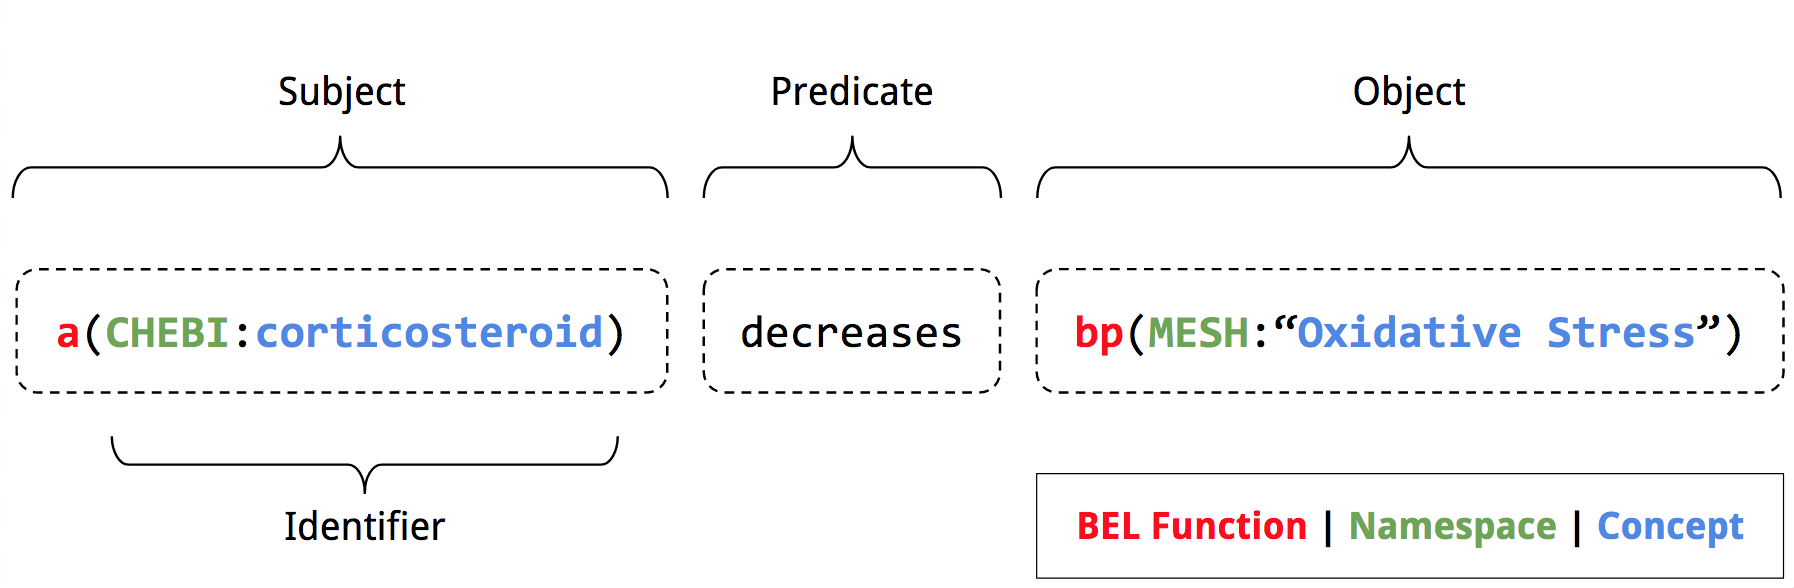
\includegraphics[width=160mm]{figures/bel_relation.png}}
    \caption[The Schema of a BEL Relation]{A BEL relation is encoded as a triplet containing a subject, a predicate, and an object. The predicate can represents the type of relation while the subject and object can either represent the abundance of molecular entities such as genes, proteins, chemicals, or more abstract concepts such as biochemical reactions, biological processes, and pathologies. Identifiers for these concepts use references to external namespaces (Figure 4B) to qualify their respective names. In this example, \ac{ChEBI}~\cite{Hastings2013} is used to qualify chemicals and \ac{MeSH}\cite{ROGERS1963} for biological processes.}
    \label{fig:bel_relation}
\end{figure}

\begin{figure}
    \captionsetup{format=plain}
    \makebox[\textwidth]{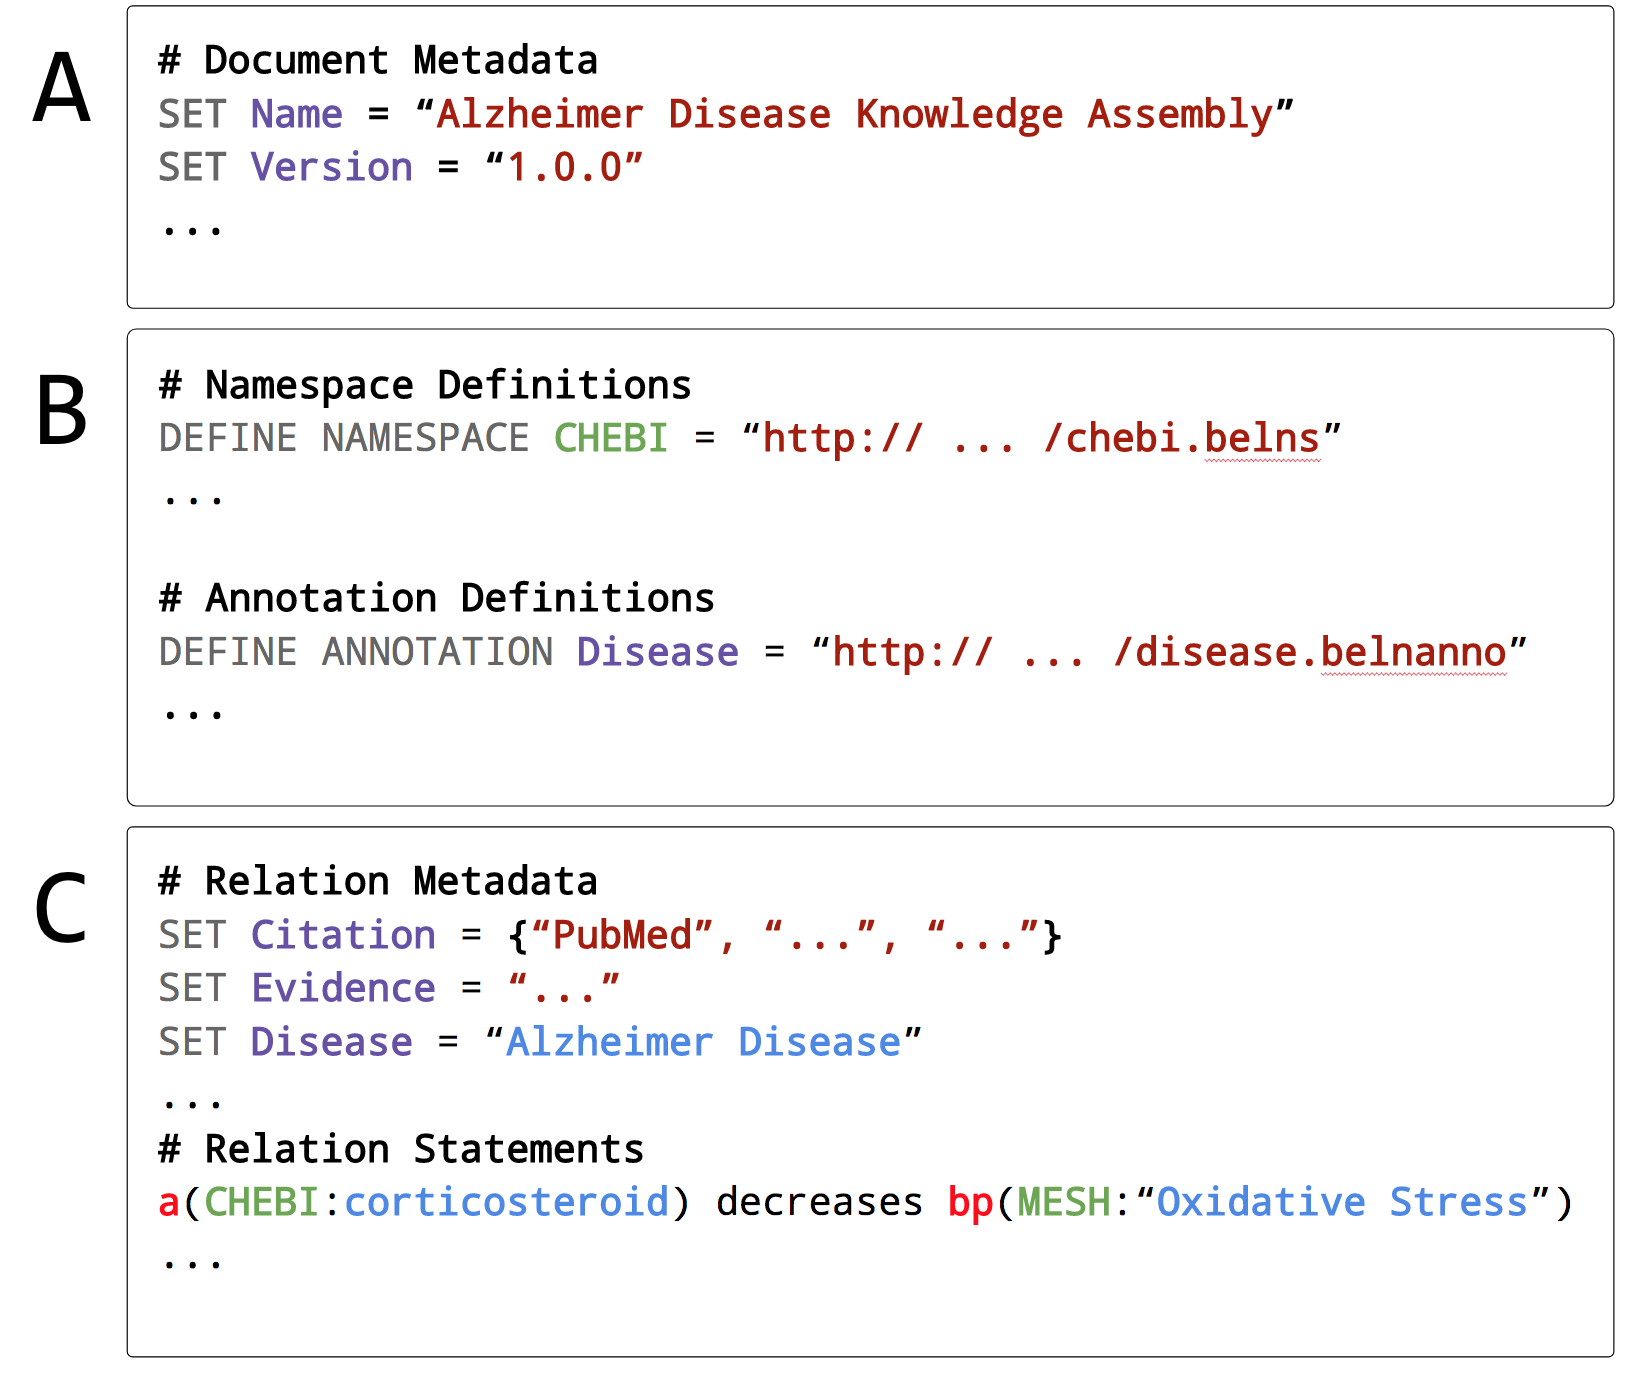
\includegraphics[scale=0.6]{figures/bel_script.png}}
    \caption[The Schema of a BEL Script]{A BEL Script contains three sections: A) the document metadata section provides provenance information such as the name, version, and author; B) the definitions section provides references to external resources that are used as identifiers and metadata in the relations section; and C) the relations section contains BEL relations and their metadata: minimally including a citation and evidence with the possibility to include additional information such as biological context (e.g., cell, anatomy, disease).}
    \label{fig:bel_script}
\end{figure}

The foray into new disease areas and clinical indications has necessitated the assembly of knowledge on wider scales from the genetic to the phenotypic and population levels.
While most modeling languages and data formats for assembling knowledge are insufficient for such a task, BEL possesses the faculty for capturing multi-scale knowledge.

In the same way \ac{BioPAX} was successful at combining many molecular pathway and interaction database, \ac{BEL} has the potential to serve as a semantic integration platform through which knowledge and data across scales can be integrated and analyzed.
\ac{BEL} can be used to reason over the previously untapped sources of chemogenomic and chemical genetic information in the realm of disease-disease, disease-protein, disease-chemical, and chemical-chemical networks.

Modeling interactions across scales is not without its issues.
As biological processes, pathologies, and phenotypes represent collections of molecular interactions, they are prone to having excessive associative and correlative relations to other biological entities.
This biases typical graph mining algorithms that rely on graph traversals to visit these types of nodes, and therefore produce less meaningful results.
While it is not within the scope of this thesis, there are many solutions for addressing these issues whose complexities vary from simple filtering to empirical traversal rules or adding extra rules for traversals.

\subsubsection{Systems Biology Graphical Notation}

\ac{SBGN}~\cite{LeNovere2009} attempts to address the inconsistency and ambiguity of current non-standardized notations for biological pathways that is problematic among \ac{BioPAX}, \ac{SBML}, \ac{BEL}, and other standardized notations.
It encompasses three variants: processes diagrams, entity relationship diagrams, and activity flow diagrams.
In a process diagram, each entity is depicted along with its transformations to other entities and the regulators of those processes.
In the entity relationship diagram, each entity appears only once and relationships are considered independent.
In the activity flow diagram, the mechanistic underpinnings are eschewed in favor of directly presenting the influence between entities.
This variant is most related to \ac{BEL} and \acp{GOCAM}, while the others are more useful for the specific mechanistic processes that are often described in \ac{SBML} models.

\subsection{Standardized Curation of Biological Knowledge}
\label{subsec:standardized_curation}

There exists thousands of biological data databases describing different biological phenomena with varying semantics and levels of granularity (Table~\ref{tab:biological_relations}).
While many have begun to use standardized ontologies and knowledge formats, many remain.
Further, the use of standard formats does not guarantee interoperability~\cite{Domingo-Fernandez2019a}.
Integrative approaches have begun to alleviate this burden for domain-specific use cases (e.g., gene set enrichment analysis on pathway and gene set databases).
In Chapter~\ref{ch:bio2bel}, a general approach for creating integrative databases using BEL is described.

\begin{table}
    \centering
    \begin{tabular}{ r l }
        Quality & Choices \\
        \hline
        Types of Relation & Causal, Correlative, Associative, Ontological \\
        Directionality of Relation & Unidirectional or Bidirectional (reflexive) \\
        Polarity of Relation & Increases, Decreases, None \\
        Causality of Relation & Direct or Indirect \\
        Modes of Entity & Activity, Abundance, Efflux  \\
        Modifications of Entity & Post-translational modifications, gene/protein fusions, mutations \\
        States of Entity & Subcellular Location, pre-/post-conditions \\

    \end{tabular}
    \caption{Examples of qualities of biological relationships and their attributes}
    \label{tab:biological_relations}
\end{table}

Further, the quantity of knowledge in the biomedical domain is increasing at an unprecedented rate — with no signs of deceleration.
Even with the assistance of information retrieval technologies, it is overwhelming, if not impossible, for individuals or groups of researchers to be knowledgeable of the state-of-the-art in any but an incredibly specific topic.
Therefore, researchers need the assistance of automated relation extraction systems to assist in the enrichment of previously existing knowledge available and integrated from relevant, high-quality databases.

The work in this thesis makes use of an ensemble of natural language processing-based, rule-based, and machine-learning based relation extraction systems through the \ac{INDRA} interface.
References to several of its constituent general purpose and biology-specific relation extraction systems are listed in Table~\ref{tab:relation_extraction_systems}.
Additionally, a sampling of BEL-specific relation extraction systems popularized by the corresponding BioCreative V BEL Task (\url{https://biocreative.bioinformatics.udel.edu/tasks/biocreative-v/track-4-bel-task}).


\begin{table}
    \centering
    \begin{tabular}{ l l l }
        Type & Name & Reference \\
        \hline
        \multirow{4}{*}{General Purpose}
        & Eidos & \url{https://github.com/clulab/eidos} \\
        & TRIPS/CWMS & \url{http://trips.ihmc.us/parser/cgi/cwmsreader} \\
        & Hume & \url{https://github.com/BBN-E/Hume} \\
        & Sofia & \url{https://sofia.worldmodelers.com/ui/} \\
        \hline
        \multirow{8}{*}{Biology-Specific}
        & TEES & \url{https://github.com/jbjorne/TEES} \\
        & REACH & \url{https://github.com/clulab/reach} \\
        & TRIPS/DRUM & \url{http://trips.ihmc.us/parser/cgi/drum} \\
        & Sparser & \url{https://github.com/ddmcdonald/sparser} \\
        & MedScan &\cite{Novichkova2003} \\
        & RLIMS-P & \url{https://research.bioinformatics.udel.edu/rlimsp}  \\
        & ISI/AMR & \url{https://githu..com/sgarg87/big_mech_isi_gg} \\
        & Geneways &\cite{Rzhetsky2004} \\
        \hline
        \multirow{4}{*}{\ac{BEL}-Specific}
        & BELIEF &\cite{Madan2016} \\
        & BelSmile &\cite{Lai2016} \\
        & BELTracker &\cite{Rastegar-Mojarad2016} \\
        & BELMiner &\cite{Ravikumar2017} \\
    \end{tabular}
    \caption{Examples of relation extraction and reading systems with varying degrees of domain specificity}
    \label{tab:relation_extraction_systems}
\end{table}

\subsubsection{Issues with Automated Relation Extraction Systems}

Neither relation extraction systems based on rules, natural language processing, nor machine learning are without their issues.
None constitute general artificial intelligence, and thus all require maintenance and improvement to sustain their abilities to process recent scientific literature; each requires increasingly large and carefully annotated corpora to support the generation of new rules or train the extraction system to recognize new relationships.

Because relation extraction systems have many subsystems with their own subtasks, the errors from each propagate throughout.
\ac{NER} remains a difficult task due to the availability and generation of supporting ontologies that precisely describe given terms.
Though it remains unpublished and tangential to the work presented in this thesis, during the course of the curation of unstructured information outlined in Chapter~\ref{ch:recuration}, an ontology was generated to capture the complex terminology surrounding the human microtubule associated protein Tau.
It was then extended during curation of other related candidate pathophysiological mechanisms of the aetiology of \ac{AD} and named the \ac{CONSO}~(\url{https://github.com/pharmacome/terminology}).
While \ac{CONSO} formalizes the terminology and discourse from the scientific literature for protein aggregation processes in several neurodegenerative diseases (e.g., Huntington's disease, \ac{AD}, \ac{PD}), it also illustrates that the large and ongoing effort required to formalize a single area of molecular biology is not easily scaled to cover all possible biology.

The realization of relation extraction systems eschews an important aspect of systems and networks biology: the biological context.
By focusing on the sentence level, it remains difficult, if not impossible, for these systems to extract the information pertaining to the cell, cell line, tissue, model organism, disease context, or other contextual information that is crucial for the understanding of complex biology.

Even with its issues, automated curation can be incredibly powerful when combined with manual curation in semi-automated workflows.
With careful generation of new terminologies, the inclusion of contextual information that can currently best be found by purely manual effort, and rational prioritization of automatically generated content for manual review, semi-automated workflows can make huge improvements in both the quantity, quality, and relevance of knowledge assembles.
Ultimately, these improvements lead to better downstream analysis as described in the following.

\section{Algorithms Applicable to Graphs}
\label{sec:algorithms}

Algorithms for analyzing pathways and networks have been placed  into three main categories by~\cite{Khatri2012}: \ac{ORA}, \ac{FCS}, and \ac{PT}.
\ac{ORA} often focuses on the number of differentially expressed genes present or absent in a gene set compared to chance, while \ac{FCS} is less susceptible to large effects and considers the aggregate of groups of small effects.
\ac{PT} finally considers the biological relations between members of the pathway during analysis.

\subsection{BEL Algorithms}
\label{subsec:bel_algorithms}

Furthermore, Martin \textit{et al.} made the distinction between methods that rely on the assumption that protein activities are correlated with their corresponding mRNAs' expression changes (forward reasoning) versus the effect that upstream controllers of mRNA expression have (backwards reasoning)~\cite{Martin2014}.
These algorithms have been developed for a wide variety of applications, data formats, and graph types.
While many are heterogeneous, below are the most notable algorithms specific to networks from knowledge assemblies encoded in BEL.

\subsubsection{Reverse Causal Reasoning}

Reverse causal reasoning (\ac{RCR}) is an approach to identify the upstream controllers of biological patterns measured in an experiment; often differential gene expression experiments between healthy and diseased patients.
First, large knowledge assemblies are dissected into smaller hypothesis networks with one upstream node with multiple outgoing causal relations to target nodes represented by the experimental data set.
Each hypothesis network is scored by its concordance between the observed up- and down-regulations of targets nodes to the sign of the causal relation and by its richness, or the explanatory power of the hypothesis network~\cite{Catlett2013}.
An example hypothesis network is shown in Figure~\ref{fig:rcr_schematic}.

\begin{figure}
\captionsetup{format=plain}
\makebox[\textwidth]{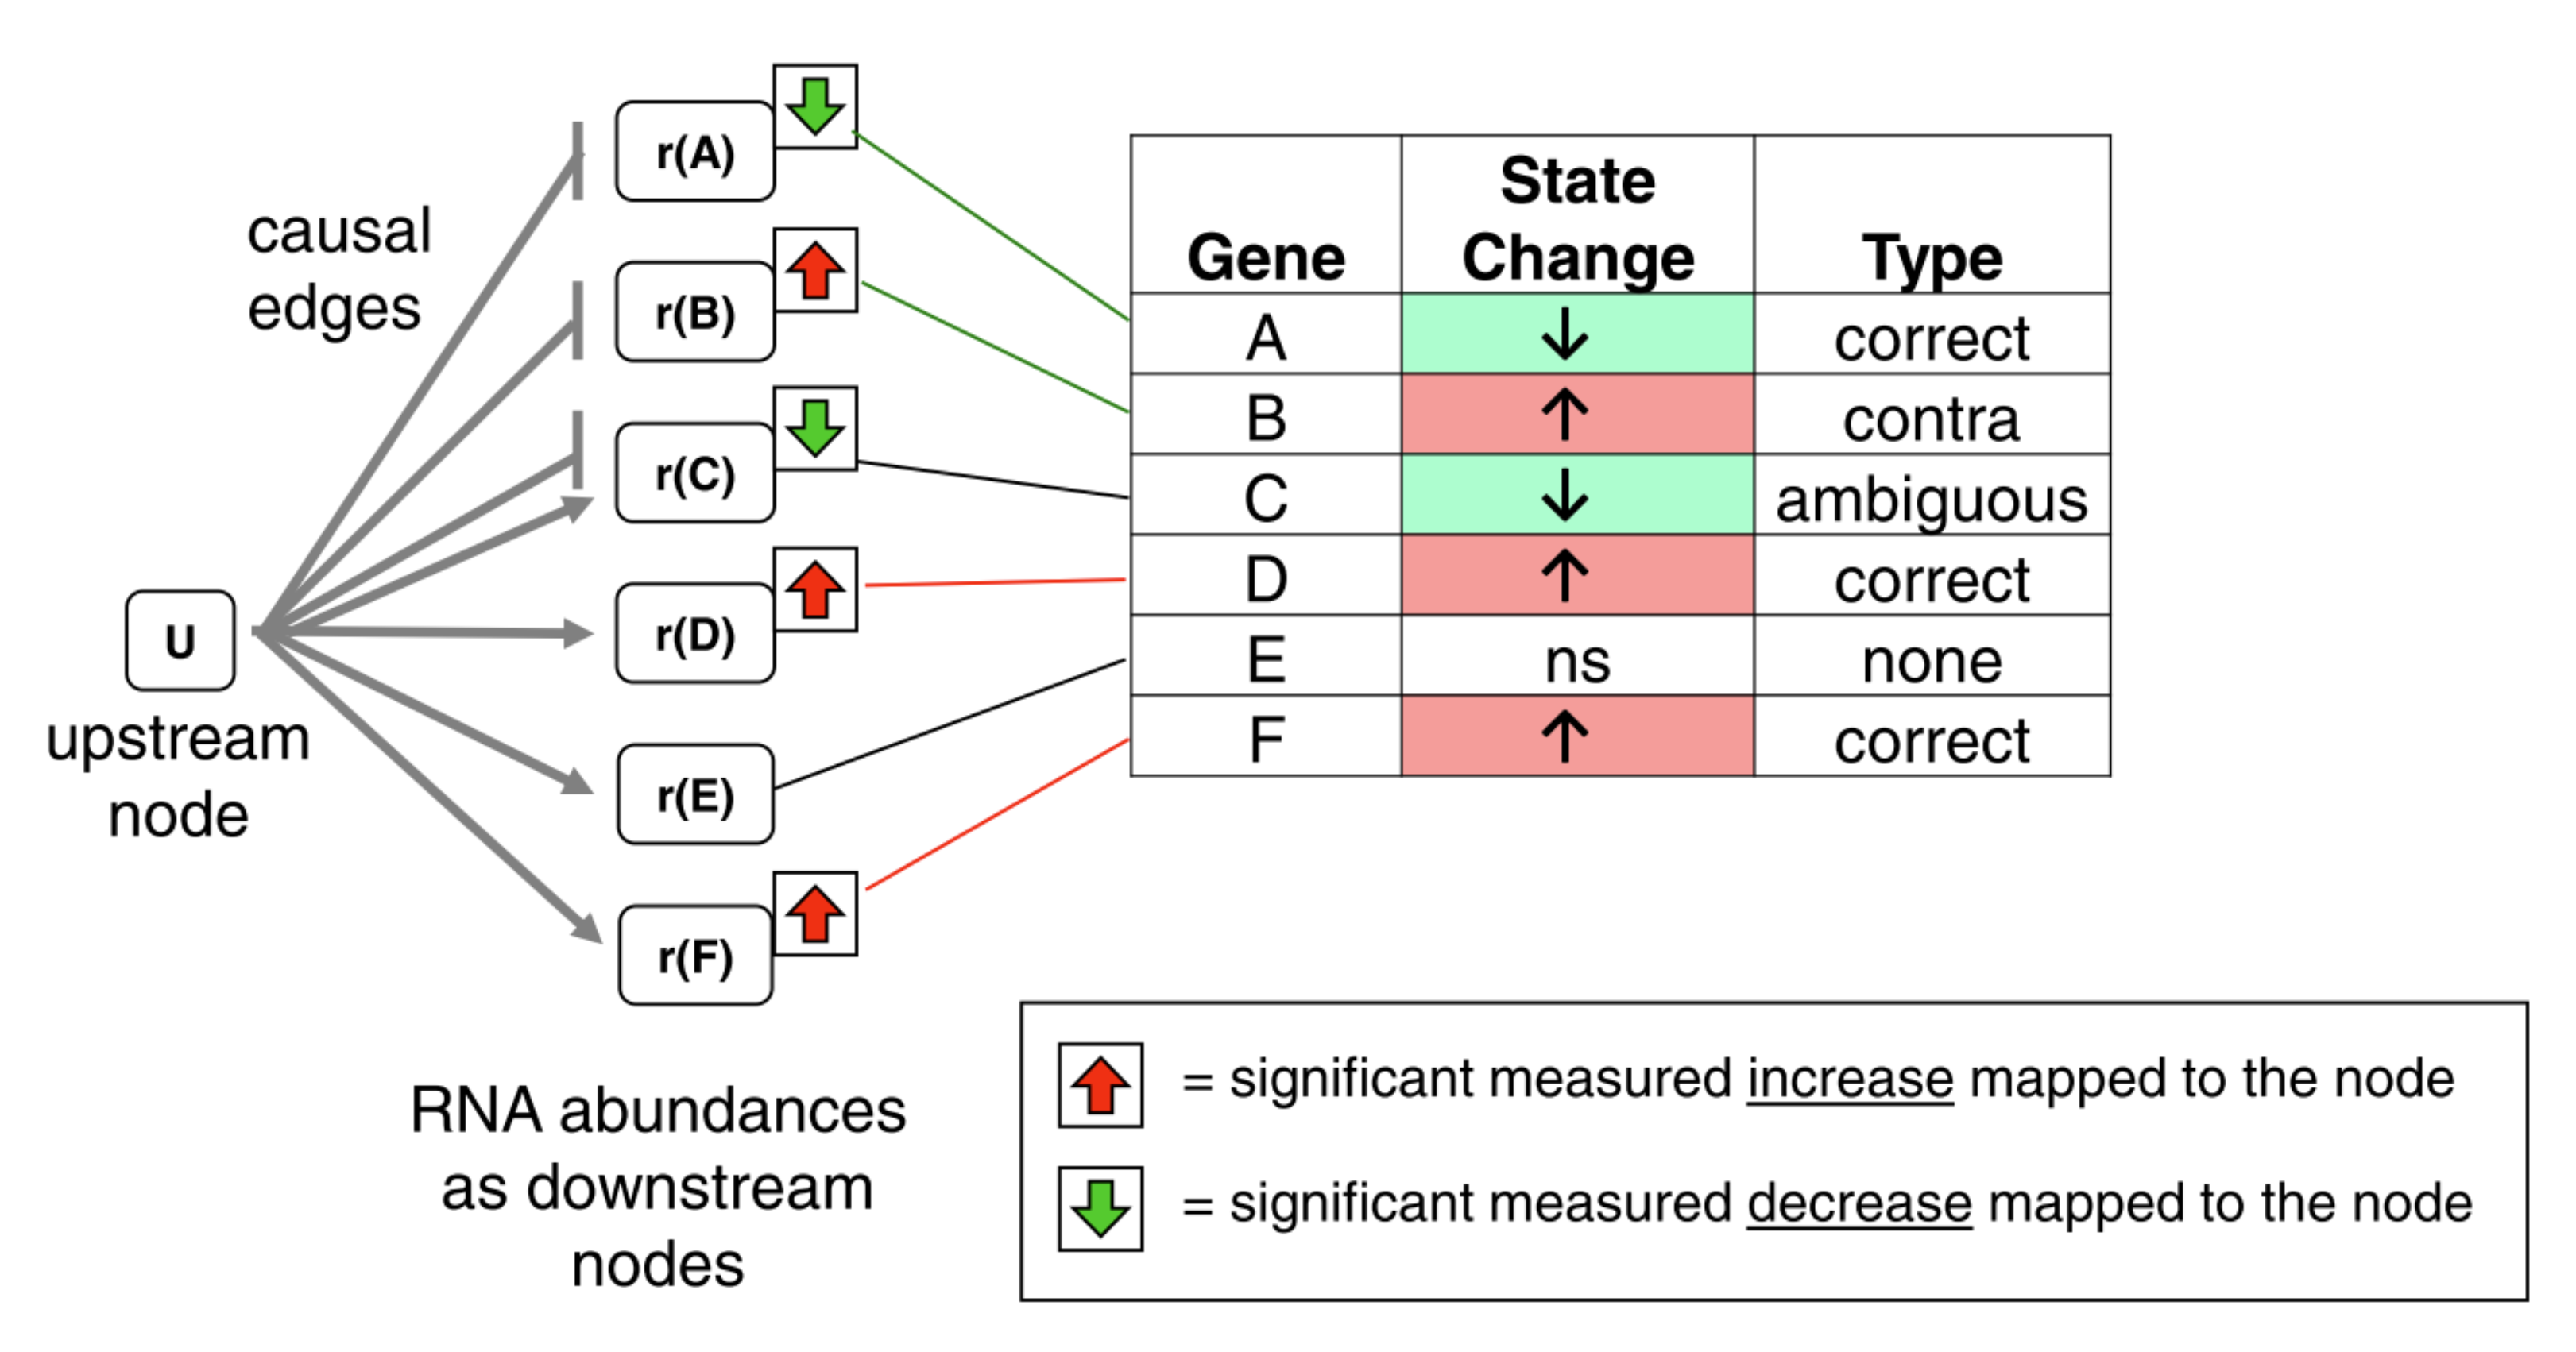
\includegraphics[width=160mm]{figures/rcr_schematic.png}}
\caption[A Schematic Diagram of \ac{RCR}]{An example hypothesis network. Target nodes are counted as correct if they have a decreasing relationship and down-regulation, or an increasing relationship and up-regulation. Target nodes with multiple conflicting relationships are marked as ambiguous. Finally, target nodes are counted as incorrect if they have a mismatch between an increasing relationship and down-regulation, or a decreasing relationship and up-regulation. Adapted from~\cite{Catlett2013}.}
\label{fig:rcr_schematic}
\end{figure}

\subsubsection{Network Perturbation Amplitude}

While \ac{RCR} gives preliminary insights to significant biological controllers, it mostly ignores the topology of signaling, regulatory, and other causal networks that can be represented in knowledge assemblies (Figure~\ref{fig:npa_schematic}).
The \ac{NPA} measures the aggregated effect explained by the controller layer with reference to a given node with respect to their downstream nodes.
Two complementary statistics for the effect of permutations of the upstream layer and downstream layer allow for further insight to the validity of \ac{NPA}s as a hypothesis generation mechanism~\cite{Martin2014}.

\begin{figure}
\captionsetup{format=plain}
\makebox[\textwidth]{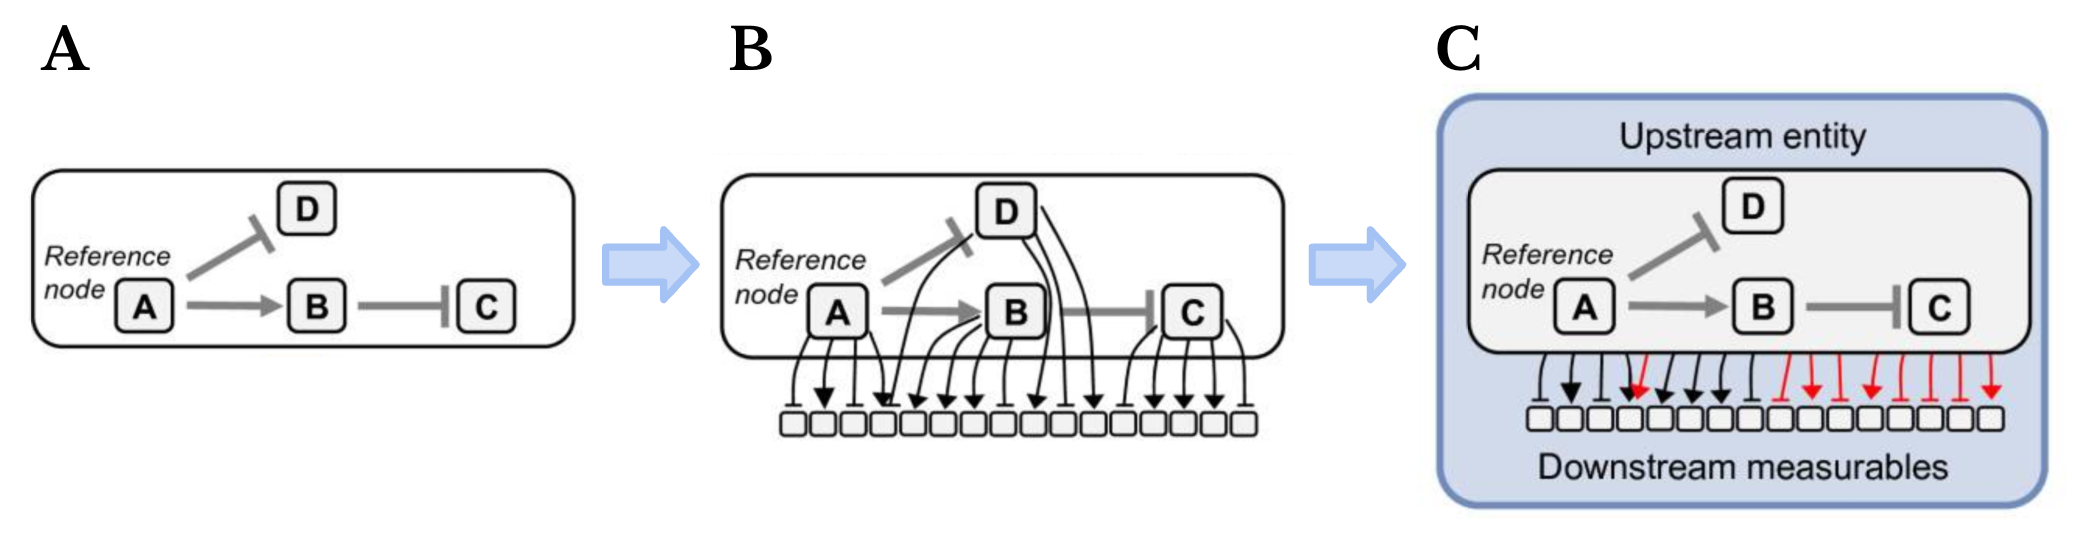
\includegraphics[width=160mm]{figures/npa_schematic.png}}
\caption[Hypothesis Network Generation for Network Perturbation Amplitude]{Creation of hypothesis networks that accounts for the topology and interactions of  upstream controller layer with respect to a reference node A), their individual effects on the downstream layer B) and their combine effect C). Adapted from~\cite{Martin2012}.}
\label{fig:npa_schematic}
\end{figure}

\subsubsection{Sampling of Spanning Trees}

While \ac{NPA} enables more informed analyses than \ac{RCR}, its mathematical basis limits the topologies of knowledge networks that can be used to those with causal consistency.
In these networks, all paths from one node to another result in the same aggregated effect of increases and decreases.
An additional approach in Figure~\ref{fig:sst_schematic} for \ac{SST} with random walkers eliminates inconsistencies and can be aggregated over multiple trials to assign \ac{NPA} scores to networks that were otherwise inconsistent~\cite{Vasilyev2014}.

\begin{figure}
\captionsetup{format=plain}
\makebox[\textwidth]{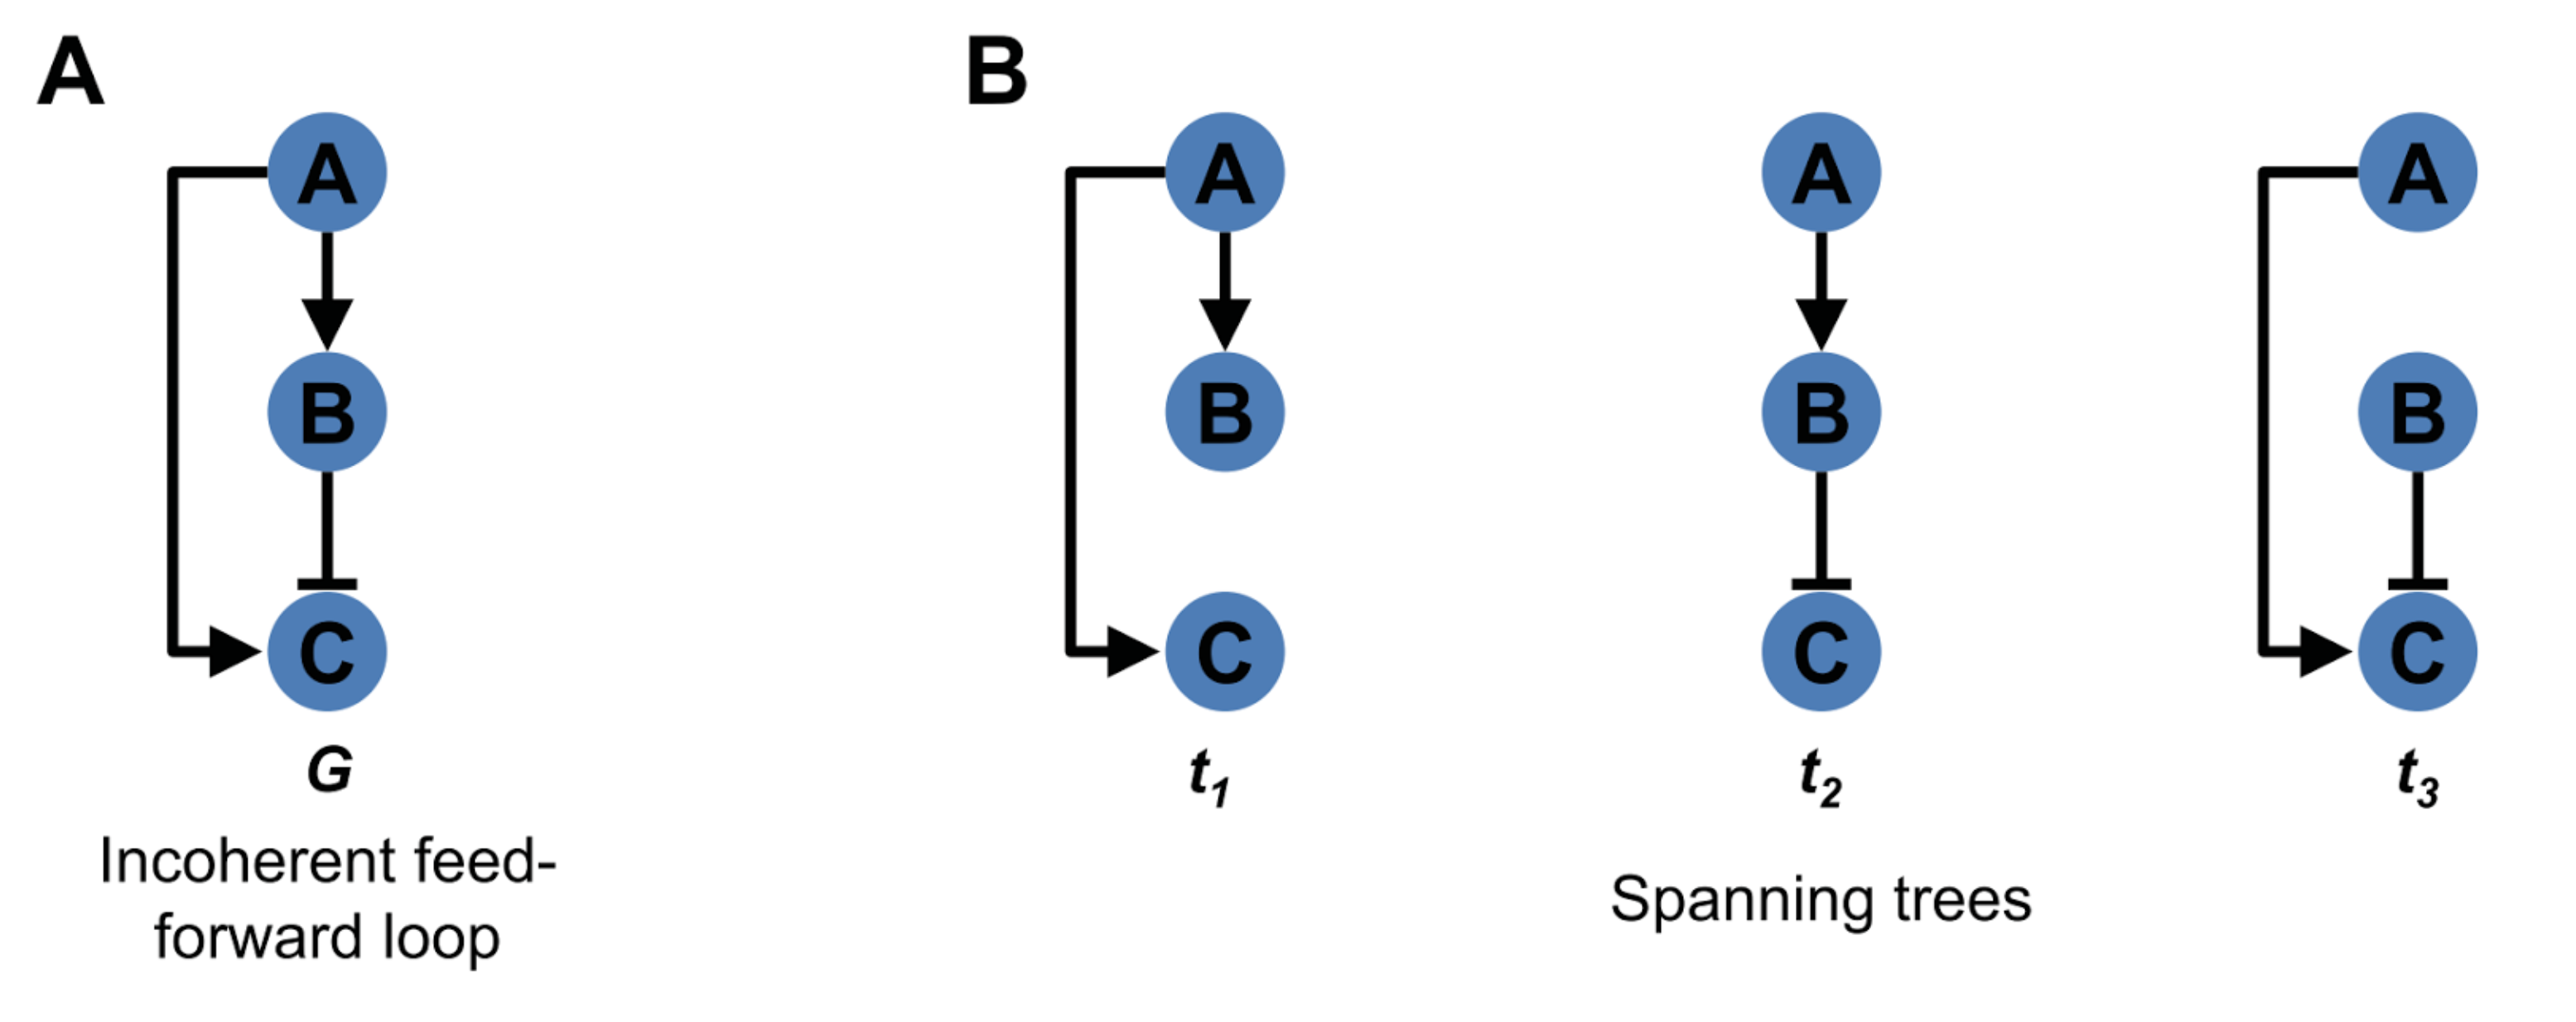
\includegraphics[width=160mm]{figures/sst_example.png}}
\caption[Decomposition of Spanning Trees]{An example decomposition of a small causally inconsistent network A) to its spanning trees B)\cite{Vasilyev2014}.}
\label{fig:sst_schematic}
\end{figure}

\subsection{Network Representation Learning}
\label{subsec:nrl}

Representation learning methods have the goal of generating low-dimensional, continuous vector representations for entities in high-dimensional, heterogeneous data sets (e.g., images, text sequences, etc.).
More specifically, network representation learning, also known as \ac{KGE}, learns representations of nodes and edges from \ac{KG}s in continuous vector spaces that can be used in downstream machine learning tasks such as edge prediction, entity clustering, and entity disambiguation~\cite{Wang2017}.
Several methods inspired by linear algebra, deep learning, and natural language processing have arisen in previous years as shown in Table~\ref{tab:kgem_examples}.

\begin{table}
    \centering
    \caption{Examples of three types of \ac{KGEM}s}\label{tab:kgem_examples}
    \begin{tabular}{ l l l }
        \hline
        Type & Model & Reference \\
        \hline
        \multirow{6}{*}{Translational Distance Models}
        & Structured Embedding & ~\cite{Bordes2011}  \\
        & TransE & ~\cite{Bordes2013} \\
        & Unstructured Model & ~\cite{Bordes2014} \\
        & TransH & ~\cite{Wang2014} \\
        & TransR & ~\cite{Lin2015} \\
        & TransD & ~\cite{Ji2015} \\
        \hline
        \multirow{4}{*}{Semantic Matching Models}
        & RESCAL & ~\cite{Nickel2011} \\
        & ERMLP & ~\cite{Dong2014} \\
        & DistMult & ~\cite{Yang2014}  \\
        & ConvE & ~\cite{Dettmers2017} \\
        \hline
        \multirow{4}{*}{Random-Walk Models}
        & DeepWalk & ~\cite{Perozzi2014} \\
        & Gat2Vec & ~\cite{Sheikh2018} \\
        & node2vec & ~\cite{Grover2016} \\
        & edge2vec & ~\cite{Gao2018} \\
        & LINE & ~\cite{Tang2015} \\
        \hline
    \end{tabular}
\end{table}

\subsubsection{Translational Distance Models}

Each translational distance model learns entity and relation embeddings in euclidean space by defining two things: 1) an equation relating the corresponding embeddings with the models' hyperparameters and 2) a distance-based measure of the plausibility of a given triple $f_r$~\cite{Wang2017}.

An example of an established translational distance model is TransE~\cite{Bordes2013}.
It models a class of relation \textit{r} as the translation from a head entity $h$ (i.e., the subject of a triple) to a tail entity $t$ (i.e., the object of a triple) in a representative euclidean space as $h + r \approx t$.
It measures the plausibility of a given the following scoring function:

\begin{equation}\label{eq:trans_e_scoring_function}
    f_r(h,t) = - \|h + r - t\|
\end{equation}

The closer the embedding of the tail is to the sum of the head and relation embeddings, the higher is the probability that the triple is correct.
However, because TransE is limited in modeling $1-N$, $N-1$, and to $N-M$ relations, several extensions have been proposed (e.g., TransH, TransR, and TransD).

\subsubsection{Semantic Matching Models}

Unlike translational distance models, semantic matching models use similarity-based scoring functions that measure the plausibility of a given triple based on the "latent semantics" of the entities and relations~\cite{Wang2017}.
An example of an established semantic matching model is RESCAL~\cite{Nickel2011}.
It represents each entity as a vector and each relation as a matrix, $M_r$, that encodes pairwise interactions between the head and tail entities of a triple, using the following scoring function:

\begin{equation}\label{eq:rescal_scoring_function}
    f_r(h,t) = h^{T} M_{r} t
\end{equation}

Both translational distance models and semantic matching models can be trained using the margin ranked loss in order to maximize the difference between true (i.e., positive) and false (i.e., negative) triples.

\begin{equation}\label{eq:margin_ranked_loss}
    L = \sum_{}^{}(f_r(h^{'},t^{'}) - f_r(h,t) + \lambda )_+,
\end{equation}

\subsubsection{Random Walk Models}

Random walk models generate embeddings for nodes in knowledge graphs by applying the concepts from natural language models (e.g., SkipGram, Word2Vec, and GloVE) to random walks.
The first, \textit{DeepWalk}~\cite{Perozzi2014}, used random walks to train a SkipGram~\cite{Mikolov2013} model in which the random walks were considered as sentences and nodes were considered as words.
Because SkipGram is a language model that maximizes the co-occurrence probability of words in the same window, the resulting node vectors reflect the local structure of the input \ac{KG} (Figure~\ref{fig:deepwalk_embedding}).
It is further rationalized by the observation that the distribution of nodes' appearances in random walks mirrors that of words in free text~\cite{Perozzi2014}.

\begin{figure}
    \captionsetup{format=plain}
    \makebox[\textwidth]{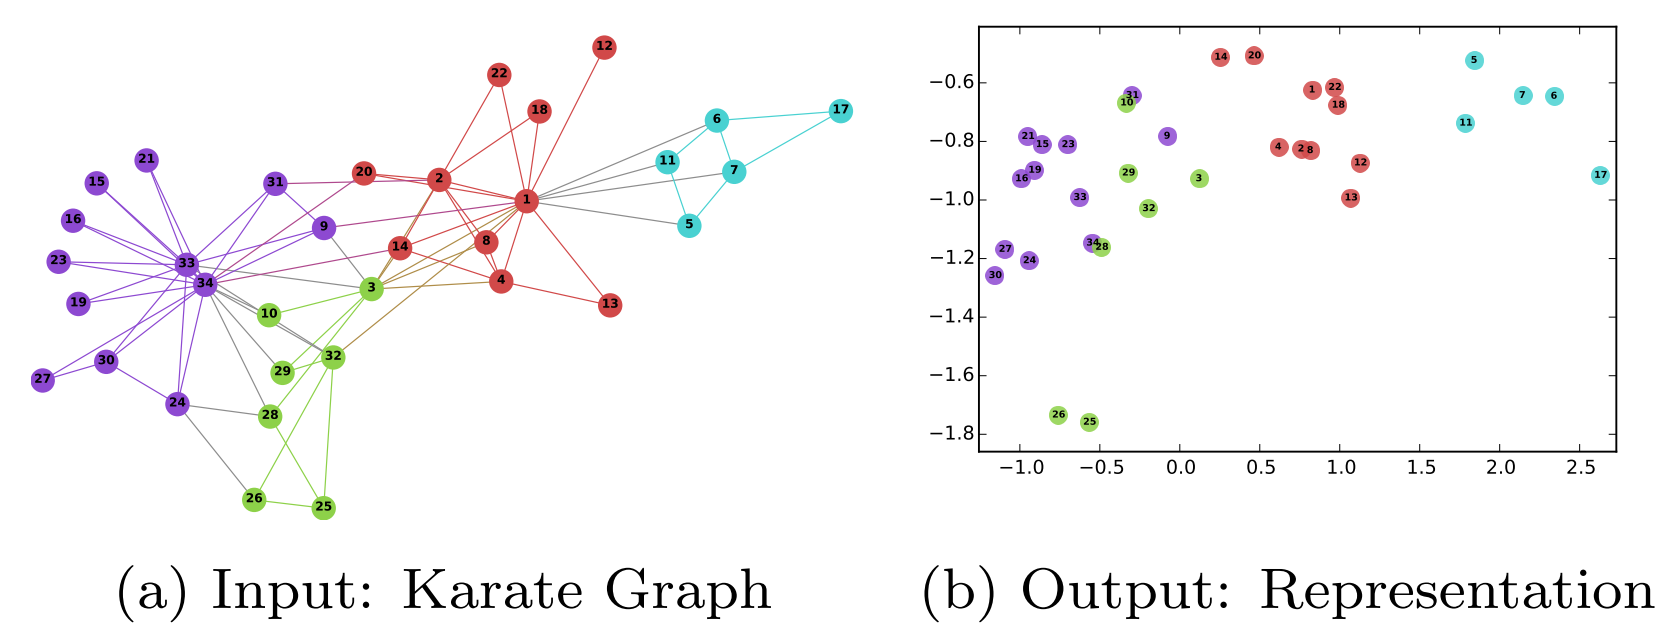
\includegraphics[width=120mm]{figures/deepwalk_embedding.png}}
    \caption{\textit{DeepWalk} produces embeddings that reflect the community structure of the underlying \ac{KG}. Figure adapted from ~\cite{Perozzi2014}}
    \label{fig:deepwalk_embedding}
\end{figure}

Biological knowledge encoded in many of the previously mentioned formats (e.g., \ac{BioPAX}, \ac{SBML}) can be directly translated into \ac{KG}s to which network representation learning can be applied.
The following subsection describes two of such applications in drug discovery.

\section{Applications}
\label{sec:introduction_applications}

While Chapters~\ref{ch:pybel},~\ref{ch:belcommons},~\ref{ch:recuration}, and~\ref{ch:bio2bel} cover the generation, enrichment, and exploration of biological knowledge graphs, Chapters~\ref{ch:bel2abm},~\ref{ch:guiltytargets}, and ~\ref{ch:epicom} cover three areas in which biological knowledge graphs can be used to support drug discovery.
While there have been many previous computational, network-based methods that have been used for these purposes, most rely on narrowly-focused databases with low granularity or slow update.
The final chapters focus on adapting these methods to higher granularity knowledge encoded in BEL for the drug repositioning task in which a new indication is proposed for a previously clinically studied chemical.
Further, these approaches can be carefully adapted for precision medicine, in which the use of a given drug should be prescribed to a given patient of subgroup of patients instead of an entire population.

\subsection{Simulation}

One of the most simple categories of biological models is boolean and logical models.
In these graphical models, nodes have boolean states that change through time based on logical rules encoded in the model.
Two prominent examples of boolean models are Petri Nets~\cite{Peterson1977} and boolean networks\cite{Albert2008}, but there have been many following successes with more complicated formulations~\cite{Saez-Rodriguez2011,Gyori2017,Karlebach2008}.

One of the most powerful simulations of biological systems comes from partial differential equations, which have the ability to precisely encode both spatial and temporal events as well as their evolution though time~\cite{Lopez2013}.
However, they suffer the drawbacks that they have a high number of unknown parameters either due to the lack of available experimental data, or due to unknown intermediate processes.
Further, fitting differential equations with high number of variables (more than several hundred) was completely inaccessible until recently.

Agent-based models provide an intermediate in which a small set of rules can be used to infer emergent properties of a system through simulation and optimization.
However, their definition is painstaking, and it is difficult to include the most relevant biological knowledge.
Chapter~\ref{ch:bel2abm} explores one way biological knowledge can be used to influence the generation and application of these types of models to understanding basic biological processes in \ac{AD}.

\subsection{Target Prioritization}

Target prioritization is the task of ranking proteins based on their relevance to a given disease and likelihood of being a successful therapeutic target.
However, it does not directly assess ligandability nor druggability, so computational approaches must be complemented by both the appropriate functional experiments (e.g., knockdown studies) and physical studies (e.g., binding assays).

A common paradigm in network analytical methods is guilt-by-association: nodes connected to similar groups of nodes have similar properties.
Many target prioritization methods use this paradigm to assume that similar proteins have similar functions and therefore candidates can be proposed on their similarity to previously known targets.
While this may limit guilt-by-association methods in their ability to prioritize novel targets, they are still considered robust~\cite{Moreau2012}.

Chapter~\ref{ch:guiltytargets} explores a novel method for calculating similarities between proteins based on network representation learning and improving the state-of-the-art pipeline presented by Emig \textit{et al.}~\cite{Emig2013}.
While initial work used the same protein-protein interaction networks and disease-specific differential gene expression profiles, it can be extended to accomodate the rich knowledge encoded in \ac{BEL} networks generated by manual, semi-automated, and automated approaches described elsewhere in this thesis.

\subsection{Mechanism of Action Deconvolution}

Understanding the mechanism of action of a given compound not only gives insight into its efficacy in a given therapeutic indication but also possible off-target effects.
Many of off-target effects may be harmful to a patient, and are often studied through the lens of toxicology~\cite{Lee2013}.
Therefore, a better mechanistic understanding might be useful not only in mitigating off-target effects but also in drug repositioning, where off-target effects are proposed as targets for other indications.
Further, investigations of the mechanism of action of a given compound have remained target-centric and have yet to access the mechanistic causal knowledge contained within biological knowledge graphs.

Network representation learning techniques are well-suited to capture patterns in compound-target pairs and can also use the high granularity mechanistic causal knowledge graphs whose generation is described in this thesis.
The embeddings generated for nodes and edges can be directly applied to the drug repositioning task by scoring the likelihood of an edge existing between a previously studied drug and a disease both existing within a network of drugs, targets, diseases, drug-target-interactions, and disease-target associations.
While this simple approach has been described in several publications, network representation learning methods allow for the easy incorporation of new entities and relation types, such as side effects and drug-side effect annotations.
Further, the constraints of drug repositioning can be related to solve the more general problem of drug discovery, which involves assessing the likelihood of the existence of an edge between any chemical and any disease.
Upcoming methods in network representation learning allow for the inclusion of literals~\cite{Kristiadi2018} into the learning process.
For biological knowledge graphs containing compounds and compound-target interactions, this enables the incorporation of chemical fingerprints into the learning process that have been previously successfully used in the fields of chemogenomics and proteochemometrics.

In order to generate efficacious therapies, mechanism of action deconvolution must be paired with knowledge about the underlying aetiological mechanisms of disease.
In the field of neurodegenerative diseases, this task is severely limited by knowledge about the diseases.
NeuroMMSig provides not only high-quality manually curated candidate mechanisms for \ac{AD}, \ac{PD}, and epilepsy as biological knowledge graphs in \ac{BEL}, but also an enrichment algorithm that goes beyond the most basic and common described by~\cite{Khatri2012} in order to incorporate the mechanistic causal information contained in the underlying knowledge graphs.

The NeuroMMSig knowledge graphs and the enrichment algorithm are used in Chapter~\ref{ch:epicom} to deconvolute the mechanism of action of the anti-epileptic, carbamazepine, that has also shown therapeutic effect in \ac{AD}.
It ranked disease-specific mechanisms in \ac{AD} and epilepsy that are likely targeted by carbamazepine and ultimately lead to the hypothesis that the GABA-ergic receptor pathway was central to its multi-indication effect.
Importantly, this investigation was advantageous over black-box machine learning models because the underlying knowledge assemblies are self-explanatory and based on publications in molecular biology and epidemiology.

Finally, the conclusion of this thesis considers the implications of moving from single targets to entire mechanisms for future drug repurposing and drug discovery, as motivated by chapters on target prioritization (Chapter \ref{ch:guiltytargets}) and mechanism of action deconvolution (Chapter \ref{ch:epicom}).

